\subsection{Comparison of Bayesian method with heuristic spot thresholding}

We have done two types of performance comparison between the Bayesian method and the heuristic spot thresholding method.

\subsubsection{Experimental data}

To test our method we have done the performance comparison between the Bayesian method and the heuristic spot thresholding method (which represents the current state-of-the-art in published CoSMoS analysis methods) on images from experimental data recordings were analyzed. The experiments were designed to produce data sets with a range of SNR in a controlled manner and with know true identity of the images as described in Methods.

Each data set was analyzed by both the Bayesian method and the heuristic spot thresholding algorithm (Figure \ref{fig:real_data}). By comparison with the known ``true'' identities of the images, the accuracy of the resulting classifications was judged using a variety of specialized statistics for binary classification data, including Recall (also known as True Positive Rate and Sensitivity), Precision, and the Matthews Correlation Coefficient (MCC) \citep{Fawcett2006-bq, Matthews1975-rw}. The MCC statistic is widely regarded as a single overall, balanced measure which is meaningful even when the classes are of very different sizes. The MCC corresponds to the Pearson correlation coefficient between the estimated and “true” binary classifications. MCC=+1 represents a perfect prediction, MCC=0 a perfectly random prediction, and MCC=-1 indicates maximal disagreement between truth and estimation. Over a range of SNR, the Bayesian method gave image classification accuracy (as quantified by the MCC) better than the heuristic spot thresholding algorithm.

\begin{figure}
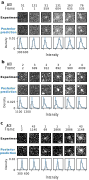
\includegraphics[width=\linewidth]{figures/figure4/figure4.png}
\caption{Performance comparison of the Bayesian method with the heuristic spot thresholding algorithm on real experimental data. (A,B) Accuracy metrics of the Bayesian analysis method (A) and heuristic spot thresholding method (B) at varying S/N of the data. (C-H) Histograms of on-target spot probabilities for each frame image calculated by the Bayesian method.}
\label{fig:real_data}
\end{figure}

\begin{figure}
\includegraphics[width=\linewidth]{figures/figure5/figure5.png}
\caption{Simulated data with varying average spot intensities ($\mu^h$). (A,B) Accuracy metrics of the Bayesian analysis method (A) and heuristic spot thresholding method (B) at varying simulated average spot intensity. (C) Average on-target spot probability (blue scatter plot) determined by the Bayesian method comparison vs the simulated average on-target spot probability (dashed line) (D-I) Histograms of on-target spot probabilities of each frame image determined by the Bayesian method.}
\label{fig:real_data}
\end{figure}

\begin{figure}
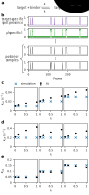
\includegraphics[width=\linewidth]{figures/figure6/figure6.png}
\caption{Simulations of data with varying average off-target spot probabilities ($\lambda^j$). (A,B) Accuracy metrics of the Bayesian analysis method (A) and heuristic spot thresholding method (B) at varying simulated $\lambda^j$. (C) Average on-target spot probability (blue scatter plot) determined by the Bayesian method comparison vs the simulated average on-target spot probability (dashed line) (D-I) Histograms of on-target spot probabilities of each frame image determined by the Bayesian method.}
\label{fig:real_data}
\end{figure}

\subsubsection{Simulated data}

In a second comparison, a series of simulated data sets were constructed for a range of signal-to-noise values. For each S/N, a set of 7,500 images (15 AoIs, 500 frames) of 14 by 14 pixels shape were generated using our probabilistic generative model. Each image is a combination of the background intensity plus randomly sampled 2-D Gaussian spots bound at the target and off-target with the intensity noise generated according to Gamma distribution.

Comparison of two methods showed similar performance on simulated data (Figure \ref{fig:simulated_data}). Taken together, these data demonstrated that the Bayesian method performs as well as or even better than the best existing CoSMoS data analysis method. Furthermore, Bayesian method achieves this performance automatically, with no adjustable parameters whatsoever, unlike the heuristic spot picker which attains this level of performance only after careful subjective trial-and-error manual adjustment of its three threshold parameters, a process that must be repeated tediously for each data set analyzed. Finally, our new Bayesian method produces a spot probability estimate for each image (not merely a Boolean spot/no spot determination) that can be used to inform subsequent kinetics calculations based on the results (e.g., the HMM analysis).

%\begin{figure}
%\includegraphics[width=\linewidth]{figures/figure5.png}
%\caption{Performance comparison of the Bayesian method with the heuristic spot thresholding algorithm on simulated data.}
%\label{fig:simulated_data}
%\end{figure}